%%
% The BIThesis Template for Bachelor Graduation Thesis
%
% 北京理工大学毕业设计(论文)第二章节 —— 使用 XeLaTeX 编译
%
% Copyright 2020-2021 BITNP
%
% This work may be distributed and/or modified under the
% conditions of the LaTeX Project Public License, either version 1.3
% of this license or (at your option) any later version.
% The latest version of this license is in
%   http://www.latex-project.org/lppl.txt
% and version 1.3 or later is part of all distributions of LaTeX
% version 2005/12/01 or later.
%
% This work has the LPPL maintenance status `maintained'.
%
% The Current Maintainer of this work is Huang Chenrui.
%%

\chapter{强化学习相关算法理论分析} % 强化学习算法理论、Q-learning、DQN、Double DQN、Dueling DQN

如图\ref{强化学习原理}所示,强化学习的基本原理在1.1节中已有提及,在此不再赘述。强化学习强调智能体与环境不断地交互,从而产生更多数据(状态和回报),并利用新的数据进一步改善自身的行为。智能体不会被告知在当前状态下,应该采取哪一个动作,只能通过不断尝试,依靠环境对动作的反馈改善自己的行为。经过数次迭代后,智能体最终能学到完成相应任务的最优动作(策略)。

本章通过对强化学习以及相关算法的理论分析,对基于值函数(Value Based)的Q-learning算法及DQN算法进行详细介绍,对DQN算法及其改进算法的优劣进行比较,选择最适合解决自动驾驶决策控制的方法。

\section{强化学习算法} % 算法的组成、选择基于值函数方法的原因、算法的求解过程。

强化学习包括智能体和环境两大对象。智能体又称为学习者或玩家,环境是指与智能体交互的内部。智能体由策略、值函数、模型三个组成部分中的一个或多个组成。下文将介绍强化学习智能体的各个组成部分与强化学习问题求解的目标,由此引出基于值函数的强化学习方法。

\subsection{强化学习算法的组成} % 谈谈为什么要选择基于值函数的方法。

(1)策略:策略是决定智能体行为的机制,是状态到行为的映射,用$\pi(a|s)$表示,它定义了智能体在各个状态下的各种可能的行为及概率。
\begin{equation}\label{pi}
    \pi(a|s) = P(A_t = a | S_t = s)
\end{equation}
策略分为两种,确定性策略和随机性策略。确定性策略根据智能体具体状态输出一个确切的动作,而随机性策略根据状态输出智能体每个动作的概率,输出值为一个概率分布。
一个策略完整定义了智能体在各个状态下的各种可能的动作及其概率大小。策略仅和当前状态有关,与历史信息无关。策略就是用来描述各个不同状态下执行各个不同行为的概率,同一时刻某一确定的策略是静态的,与时间无关,但是智能体可以随着时间更新策略。

(2)值函数:值函数代表智能体在给定状态下采取某个行为的好坏程度。这里的好坏用未来的期望回报表示,而回报和采取的策略有关,所有值函数的估计都是基于给定的策略进行的。值函数(或称为回报)用$G_t$表示,也称为“收益”或“奖励”。
\begin{equation}\label{G_t}
    G_t = R_{t+1} + \gamma R_{t+2} + \gamma^2 R_{t+3} + \dots = \sum_{k=0}^\infty \gamma^k R_{t+k+1}
\end{equation} 
其中折扣因子$\gamma$(衰减系数)体现了未来的回报在当前时刻的价值比例,在$k+1$时刻获得的回报$R$在$t$时刻体现出的价值是$\gamma^k R$。$\gamma$接近0表示趋向于当前利益;$\gamma$接近1表示偏向于长远期的利益。

值函数分为状态值函数与状态行为值函数,二者都与回报有关。

状态值函数$V_{\pi}(s)$表示从状态$s$开始,遵循当前策略$\pi$所获得的期望回报。
\begin{equation}
    \begin{aligned}
        V_{\pi}(s) &= E_{\pi}[G_t | S_t = s]\\
                     &= E_{\pi}[R_{t+1} + \gamma R_{t+2} + \gamma^2 R_{t+3} + \dots | S_t = s]\\
    \end{aligned}
\end{equation}

值函数的另一个类别是状态行为值函数$Q_{\pi}(s,a)$,也称为行为值函数。该函数表示针对当前状态$s$执行某一具体行为$a$后,继续执行策略$\pi$所获得的期望回报;也表示遵循策略$\pi$时,对当前状态$s$执行行为$a$的价值大小。
\begin{equation}
    \begin{aligned}
        Q_{\pi}(s,a) &= E_{\pi}[G_t | S_t = s, A_t =a]\\
                     &= E_{\pi}[R_{t+1} + \gamma R_{t+2} + \gamma^2 R_{t+3} + \dots | S_t = s, A_t =a]\\
    \end{aligned}
\end{equation}

(3)模型:在强化学习任务中,模型是智能体对环境的一个建模。环境模型至少要解决两个问题,一是预测状态转移概率$P_{ss^{'}}^a$,即预测在状态$s$上采取行为$a$后,下一个状态$s^{'}$的概率分布;二是预测在状态$s$上采取行为$a$后可能获得的立即回报$R_s^a$。
\begin{equation}
    \begin{aligned}
        & P_{ss^{'}}^a = P(S_{t+1} = s^{'} | S_t = s, A_t = a) \\
        & R_s^a = E[R_{t+1} | S_t = s, A_t = a] \\
    \end{aligned}
\end{equation}
根据智能体在与环境交互的过程中是否建立环境的模型,强化学习可以分为两个大类,即有模型方法和无模型方法。
一般的模型已知问题,就是智能体获得了确切的状态转移概率$P_{ss^{'}}^a$和回报$R_s^a$。

在后续章节的仿真环境介绍中,由于车辆的决策控制较难采用已知模型(如动力学模型、运动学模型)进行刻画,故均使用“无模型方法”的假设,即智能体在整个训练过程中不需要对环境模型进行建模,直接使用学习得到的经验进行策略的优化。

根据以上三点概念,可以通过建立状态值估计的方法或建立策略估计的方法来解决强化学习问题。基于值函数的方法在求解强化学习的目标时只估计状态值函数,不估计策略函数,最优策略函数在对值函数进行迭代求解时,通过状态值函数间接得到。针对自动驾驶避障问题,由于我们较难估计车辆状态与行为之间的映射(即策略函数),但可以估计车辆在采取某个动作时,车辆状态发生的变化和环境回报(即状态值函数),所以采取基于值函数的方法更加符合解决自动驾驶避障问题所需要达成的目标。

\subsection{强化学习算法的求解} % 谈谈求解强化学习算法需要什么(仿真环境[抽象问题] + 算法网络)           % TODO:这里要不要绘制一个马尔科夫决策链放附录?

求解强化学习问题的目标是求解每个状态下的最优策略,即在运行过程中接收的累计回报最大。为了获取更高的回报,智能体在进行决策时要考虑立即回报,也要考虑后续状态的回报。解决强化学习问题一般需要两步,将实际场景抽象成一个数学模型,然后去求解这个数学模型,找到使得累计回报最大的解。

第一步:构建强化学习的数学模型——马尔科夫决策(Markov Decision Process, MDP)\cite{monahan1982state}模型。

不论涉及的智能体结构、环境和交互细节多么复杂,此类交互问题都能简化为三个信号:智能体的行为、环境的状态、环境反馈的回报。具体到实验中,便是仿真环境根据智能体做出的行为产生的回报和改变的状态。马尔科夫决策模型可以有效表示实际的强化学习问题,这样解决强化学习问题的问题就转化为求解马尔科夫决策模型的最优解。

第二步:求解马尔科夫决策模型的最优解。

求解马尔科夫决策问题,是指求解每个状态下的行为,使得累计回报最大。对于环境已知的情况可以选用基于模型的方法如动态规划法;基于未知的情况选择无模型方法如时序差分法;对于状态空间、动作空间连续的场景可以采用值函数逼近法等等。根据2.1.1节的分析,如何求解马尔科夫决策模型便是具体的算法与网络结构,下文将对基于值函数(Value Based)的Q-learning算法及DQN算法进行详细介绍。

\section{Q-learning算法} % 先讲时序差分TD,再讲Q-learning。

在介绍Q-learning算法之前,首先对时序差分方法进行简单的介绍。时序差分学习最早由A.Summuel在跳棋算法中提出,1988年,Sutton证明了时序差分方法在最小均方误差(MSE)上的收敛性\cite{1998Reinforcement},之后时序差分方法被广泛应用在无法产生完整轨迹的无模型强化学习问题上。时序差分(TD)方法是无模型方法,无法获得当前状态的所有后续状态及回报,仅能通过采样学习轨迹片段,用下一状态的预估状态价值更新当前的状态价值。

Q-learning算法属于离线策略时序差分(TD)问题,最早由Watkins和Dayan在1992年提出\cite{1992Technical},其任务是通过不断地学习,不断的更新状态-动作值函数$Q(s,a)$,从而得出最优策略。根据2.1.2节中所提到的,求解强化学习问题的目标是求解每个状态下的最优策略,Q-learning算法在更新一个状态-动作值函数(以下简称Q值)时,采用的不是遵循当前策略(行为策略$\mu$)的下一个状态-动作对的Q值,而是待评估策略(目标策略$\pi$)产生的下一个状态-动作对的Q值。更新公式如下:
\begin{equation}\label{Q-learning}
    Q(S_t, A_t) \gets Q(S_t, A_t) + \alpha (R_{t+1}+\gamma Q(S_t, A^{'}) - Q(S_t, A_t))
\end{equation}
其中$\alpha$称为学习率,$\gamma$称为折扣因子,TD目标$R_{t+1}+\gamma Q(S_t, A^{'})$是基于目标策略$\pi$产生的行为$A^{'}$得到的Q值和一个立即回报的和。在Q-learning算法中,行为策略$\mu$是基于原始策略的$\epsilon$-贪心策略,保证取得经历足够丰富的新状态。目标函数$\pi$是单纯的贪心策略,通过最大化TD目标来保证策略最终收敛到最佳策略。

Q-learning算法处理有限的状态空间与有限的动作空间的问题,状态值和动作放在Q表中,值函数能够表示为一个数组。但在实际情况下,强化学习面临的问题的状态空间往往是连续的,无法用表格的方法准确列出每一种状态对应的Q值大小,故需要进行对Q值进行非线性的逼近。下文的DQN就属于这样的方法。无论是Q-learning或是DQN,均采用了目标策略$\pi$产生的下一个状态-动作对的Q值对原有的Q值进行更新,这是时序差分法的一般思想。

Q-learning的算法流程如下:

\begin{algorithm}[H]  
	\caption{Q-learning算法}%算法名字
	\KwIn{环境$E$,状态$S$,动作$A$,折扣因子$\gamma$,学习率$\alpha$,初始化行为值函数$Q(s,a)=0$}%输入参数
	\For{k = 0,1,2,\dots,m}{
		初始化状态s\;
		\For{t=0,1,2,\dots}{
            在$E$中通过$\pi$的$\epsilon$-贪心策略采取行为$a$\;
            $r$,$s^{'}=$在$E$中执行动作$a$产生的回报和转移的状态\;
            $Q(S_t, A_t) \gets Q(S_t, A_t) + \alpha (R_{t+1}+\gamma Q(S_t, A^{'}) - Q(S_t, A_t))$\;
            $s \gets s^{'}$\;
        }
	}
    $\pi^{*}(s) = \arg \max_{a \in A} Q(s,a)$\;
    \KwOut{最优策略$\pi^{*}$}%输出
\end{algorithm}

\section{DQN算法} % DQN网络图+较为具体的实现。

DQN(Deep Q-Network)算法是建立传统强化学习算法Q-learning的基础上的时序差分算法,Q-learning是离线策略时序差分法,使用$\epsilon$贪心策略产生数据,利用查表法对行为值函数(Q值)进行预测,TD目标是$R_{t+1}+\gamma Q(S_t, A^{'})$。DQN算法在传统强化学习Q-learning的基础上,主要对其精确的查表法做了近似拟合,同时通过引入深度学习网络,对网络结构和参数更新做出了如下改进。

(1)DQN使用深度神经网络从原始数据中提取特征,近似行为值函数(Q值)。

当状态空间很大且连续时,无法使用查表法来求解每个状态的价值,此时可以考虑“离散”状态空间的方法来减少算力。在“离散”状态空间中,使用深度神经网络来表示行为值函数是常见的方法。对于深度神经网络,其参数是每层网络的权重及偏置,用$\theta$表示,对值函数的更新等价于对参数$\theta$的更新。DQN神经网络结构如图\ref{DQN神经网络结构}所示。

DQN神经网络结构是三个卷积层和两个全连接层。输入为经过处理的4个连续的84$\times$84的图像,经过卷积层和两个全连接层输出包含每一个动作的Q值向量。DQN网络将高维的状态输入转换为低维的动作输出,即将图像输入转换为动作输出。利用深度神经网络实现了数据的降维。

\begin{figure}[htbp]
    \vspace{13pt} % 调整图片与上文的垂直距离
    \centering
    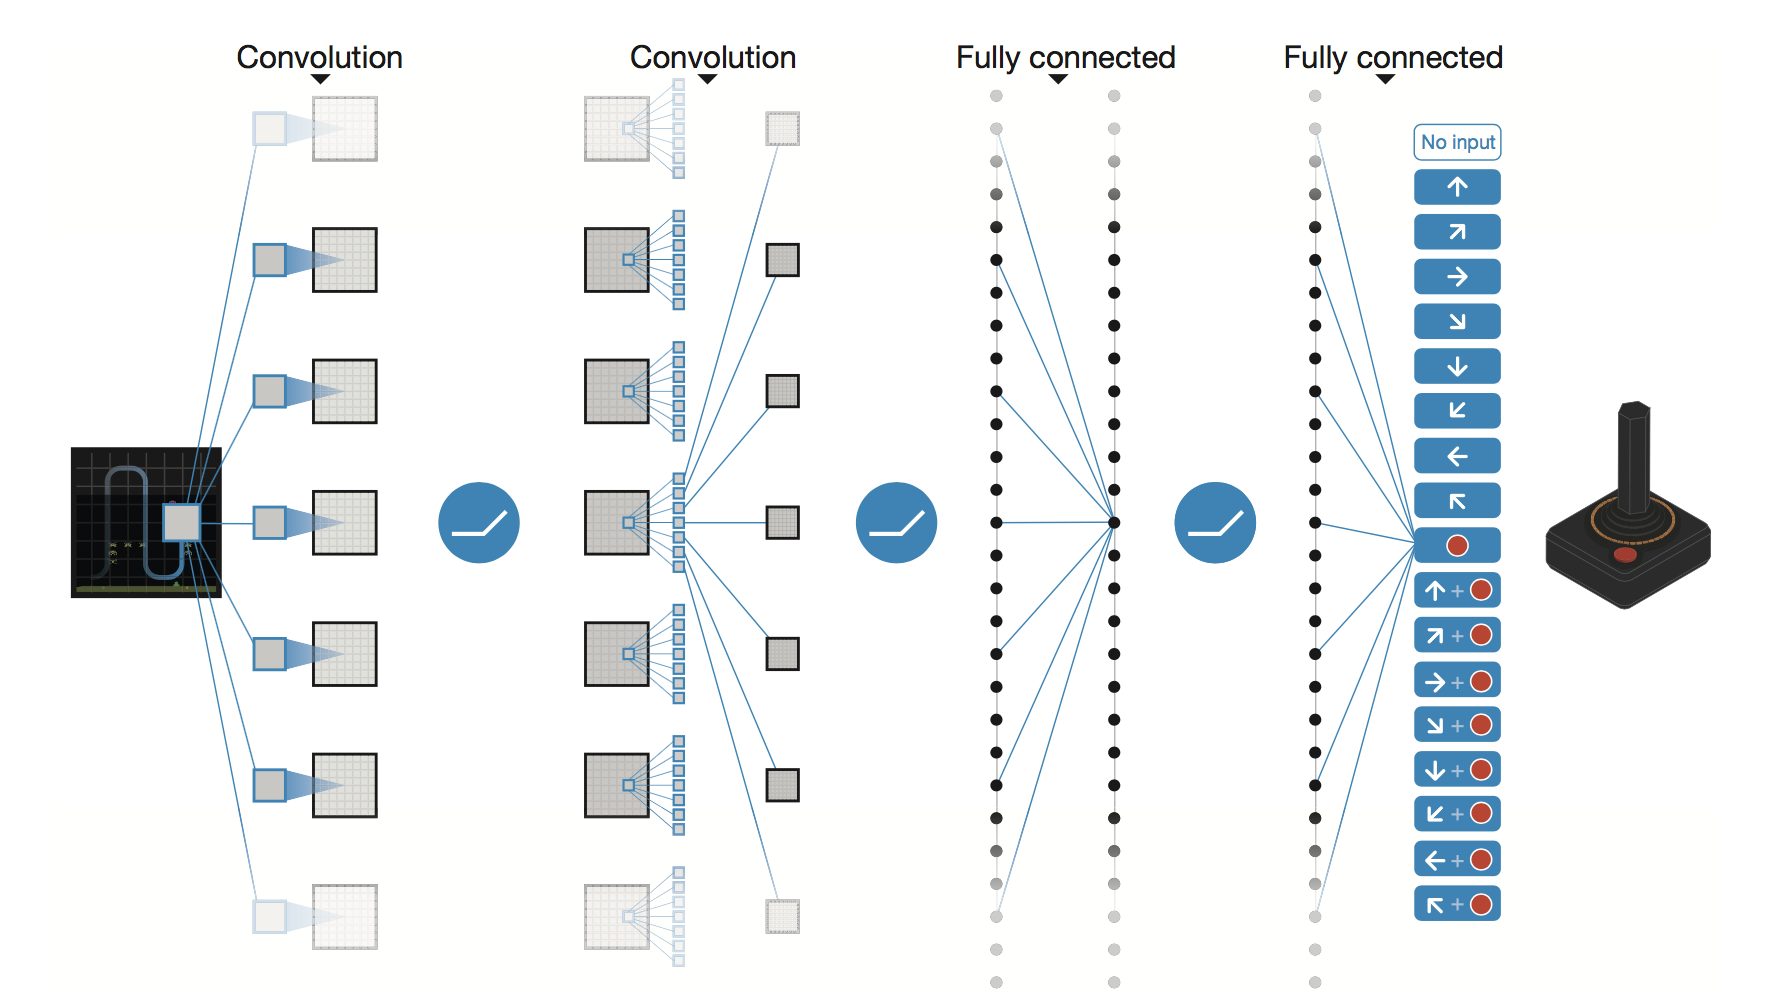
\includegraphics[width=0.73\textwidth]{images/chapter2/DQN_model.png}
    \caption{DQN神经网络结构}\label{DQN神经网络结构} % label 用来在文中索引
\end{figure}

(2)DQN使用经历回放训练强化学习。

在使用深度神经网络进行行为值函数(Q值)近似时,如果不对训练数据做处理,直接将当前时刻的信息进行学习训练,学习效果会出现较大偏差。由于使用神经网络的前提是数据之间独立同分布,而强化学习过程中,数据是通过与环境交互产生的,相邻数据之间高度相关。如果智能体在很长一段时间均学习相同环境下的数据,在接收到另一环境的数据后,参数会出现不稳定与大范围波动发散,求解无法收敛。针对这一问题,DQN采用“经验回放”的方法进行解决。

\begin{figure}[htbp]
    \vspace{13pt} % 调整图片与上文的垂直距离
    \centering
    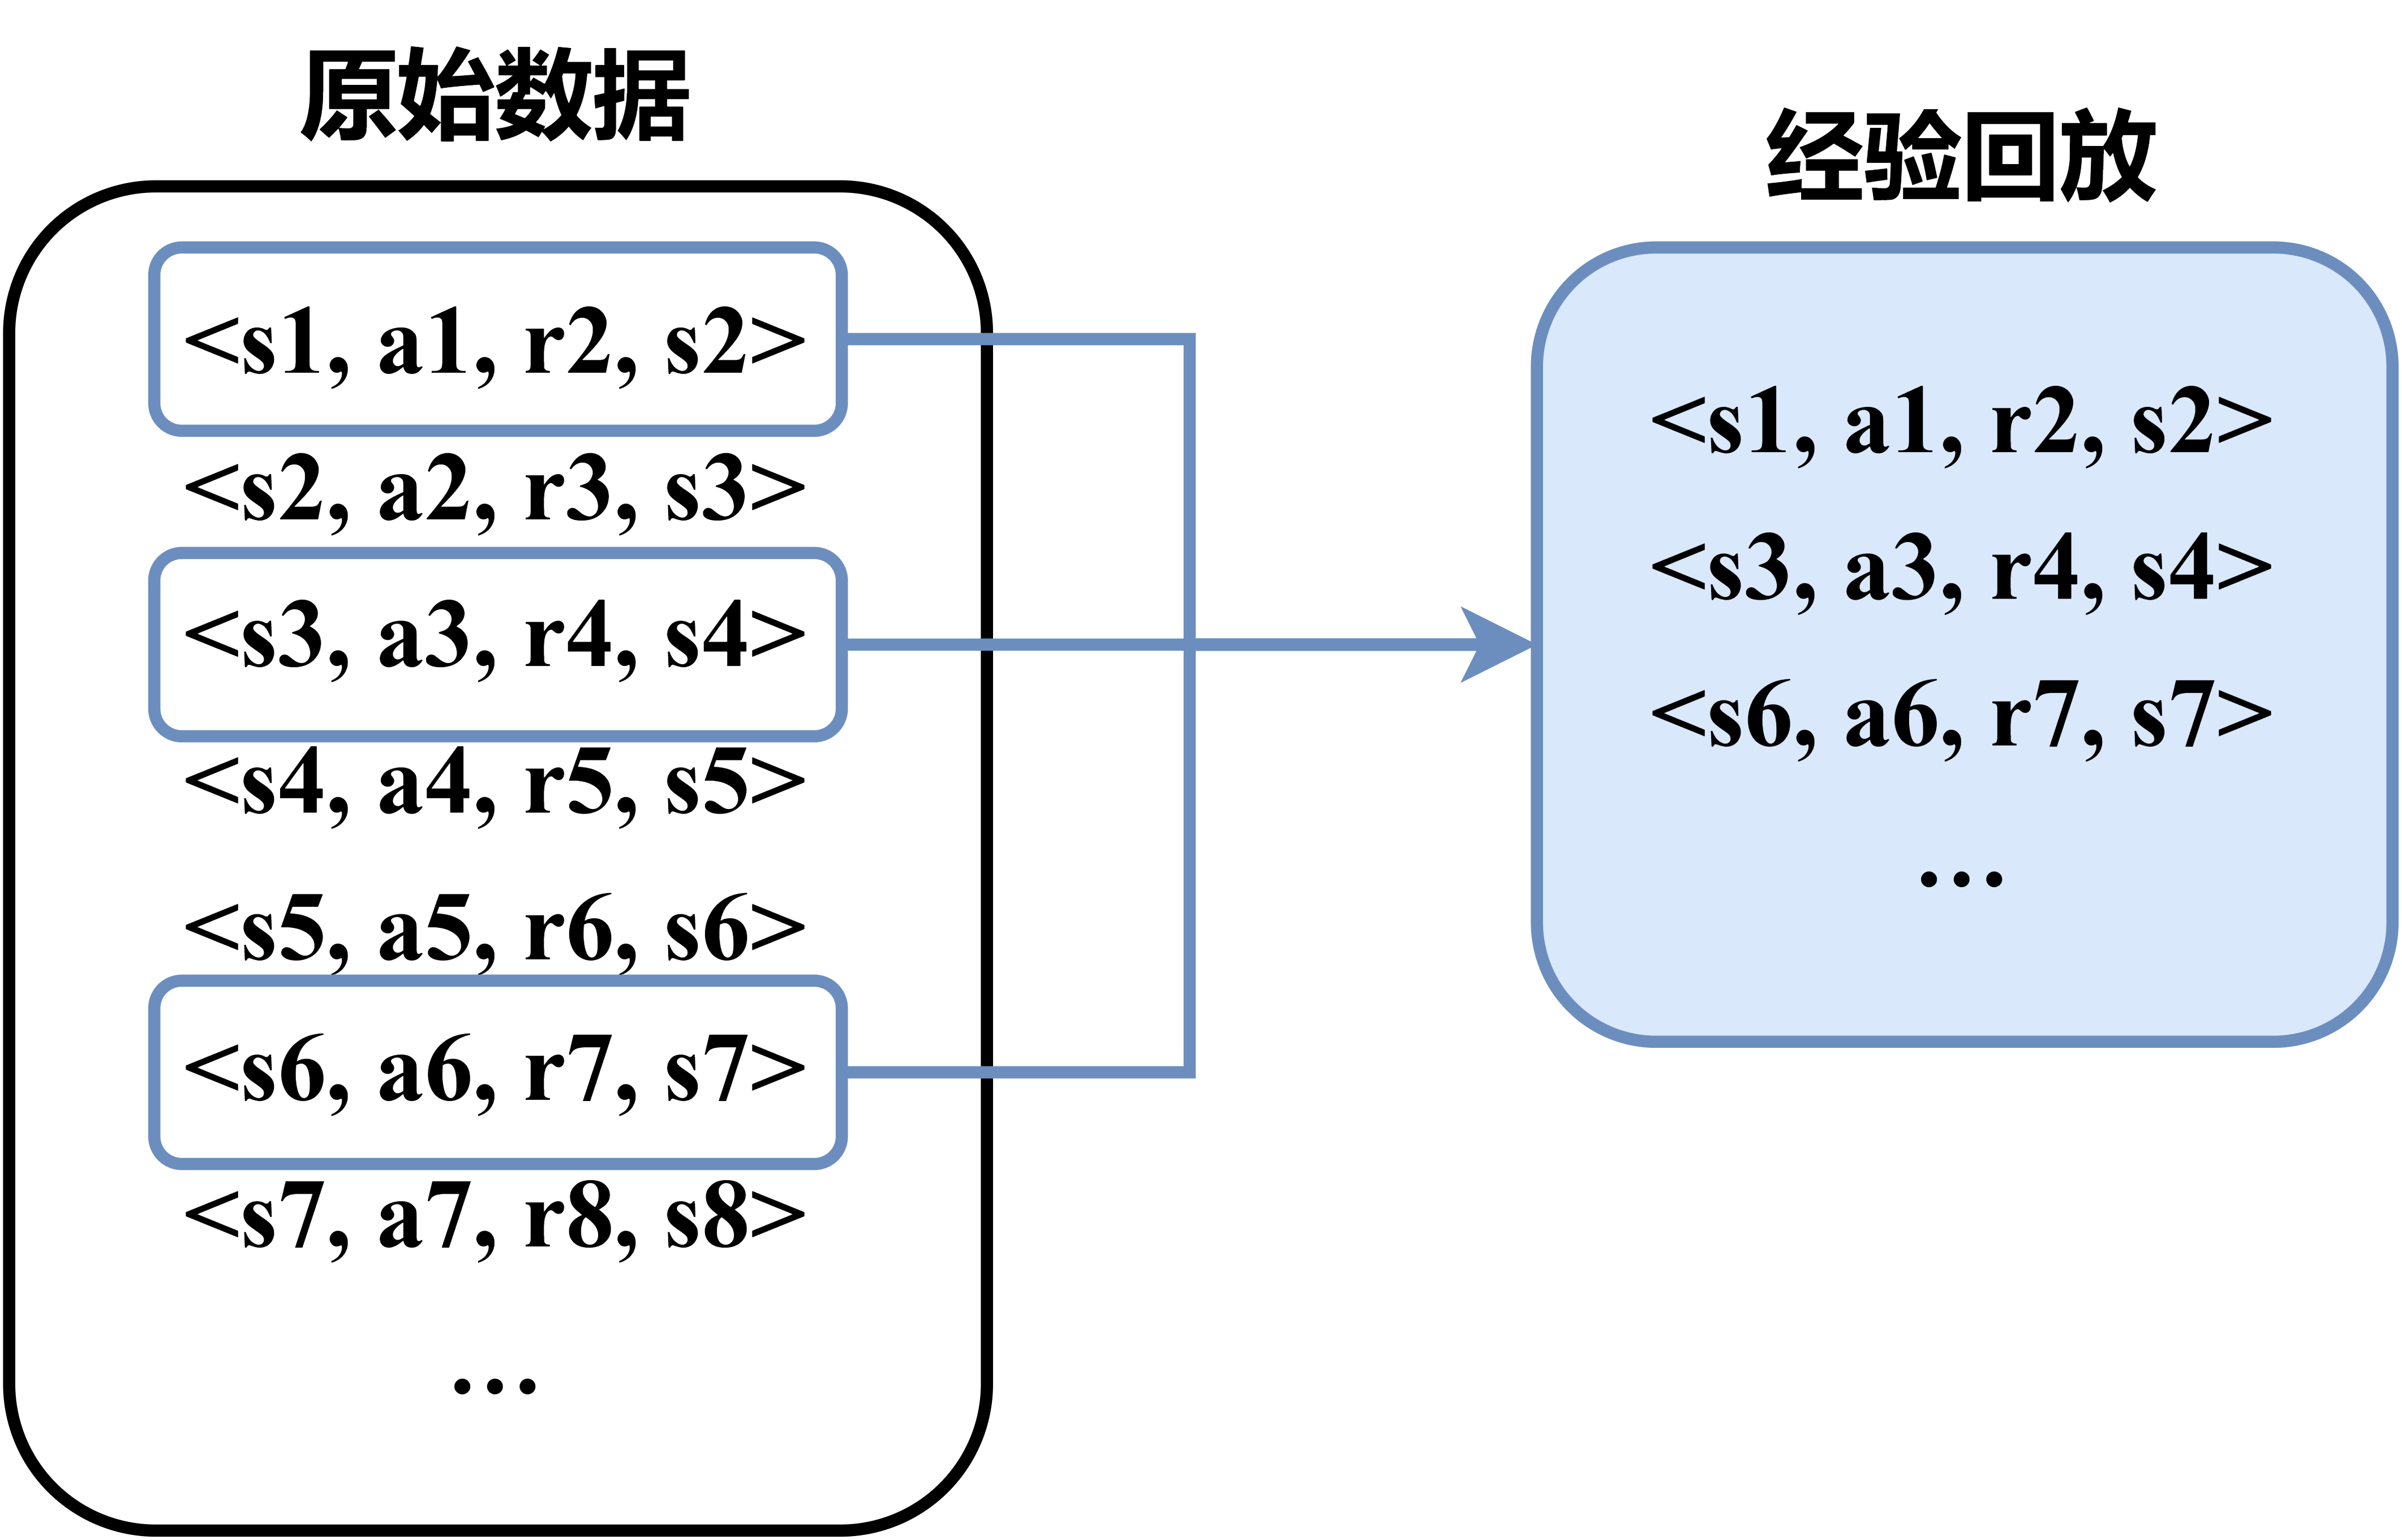
\includegraphics[width=0.63\textwidth]{images/chapter2/Experience_Replay.png}
    \caption{经验回放}\label{经验回放} % label 用来在文中索引
\end{figure}

经验回放最早由Long Ji Lin在1993年提出\cite{1992Reinforcement},如图\ref{经验回放},它在强化学习中是这样实现的:智能体跟环境不断交互,将在环境中积累的数据存储到记忆库中。首先对环境做出探索并将<本时刻状态、行为、奖励、下一时刻状态>($<s_1, a_1, r_2, s_2>$)作为一个事件对进行存储,每一次对神经网络中的参数进行更新时,利用均匀随机采样的方法从数据库中抽取数据,通过抽取的数据对神经网络进行训练。因为经验回放的样本是随机抽取,每次用于训练的样本不再是连续的数据,打破了数据的关联,由此可以满足神经网络的假设要求。

(3)DQN使用单独的目标网络处理TD偏差。

与式\ref{Q-learning}类似,DQN更新神经网络的参数$\theta$采用的是梯度下降法。更新公式如下:
\begin{equation*}
    \theta_{t+1} = \theta_t + \alpha (r + \gamma \max_{a^{'}} Q(s^{'}, a^{'}; \theta_t) - Q(s, a; \theta_t))\nabla   Q(s, a; \theta_t)
\end{equation*}

但如(2)中提及,行为值函数($Q(s, a; \theta_t)$)和TD目标值函数($r + \gamma \max_{a^{'}} Q(s^{'}, a^{'}; \theta_t)$)产生的数据需要避免关联性。为解决上述问题,DQN引入两个神经网络,一个网络固定参数专门用来产生TD目标,称为TD网络。另一个网络专门用来评估策略更新函数,逼近值函数,称为行为值函数(Q值)逼近网络。两个网络参数的更新速率不一致,用于行为值函数(Q值)逼近的网络参数每一步都更新;用于计算TD目标值的网络参数每隔固定的步数更新一次,期间保证不变。于是得到以下DQN网络的更新公式:
\begin{equation}\label{DQN}
    \theta_{t+1} = \theta_t + \alpha (r + \gamma \max_{a^{'}} Q(s^{'}, a^{'}; \theta_t^{-}) - Q(s, a; \theta_t))\nabla   Q(s, a; \theta_t)
\end{equation}

综合上述三点改进,DQN算法将经验回放和设置单独的目标网络两个方面对Q-learning方法进行改善,使其对于更加复杂的问题和大规模神经网络更加稳定和容易收敛,DQN的算法流程如下:

\begin{algorithm}[H]  
	\caption{DQN算法}%算法名字
	\KwIn{环境$E$,状态$S$,动作$A$,折扣因子$\gamma$,学习率$\alpha$}%输入参数
	初始化经验回放库D并定义容量N\;
    随机初始化网络参数$\theta$,用$\theta$初始化主网络$Q(; \theta)$\;
    随机初始化网络参数$\theta^{-}=\theta$,用$\theta^{-}$初始化TD网络$Q(; \theta^{-})$\;
    \For{k = 0,1,2,\dots,m}{
		初始化状态s\;
		\For{t=0,1,2,\dots}{
            在$E$中通过主网络的$\epsilon$-贪心策略采取行为$a$(以$\epsilon$概率随机选择任一随机动作,以$1-\epsilon$概率选择行为值函数最大的动作,即$a = \arg \max_{a \in A} Q(s,a; \theta)$\;
            在$E$中执行动作$a$,返回奖励$r$,和下一时刻状态$s^{'}$\;
            将当前事件对$<s,a,r,s^{'}>$存入经验回放库D中\;
            从经验回放库D中随机采样$n$个数据,进行如下算法更新:\
            $
                q_{target} = 
                \begin{cases}
                    r , &end\\
                    r + \gamma \max Q(s^{'},a;\theta^{-} ), &else
                \end{cases}
            $
            \\
            $
                q_{next} = Q(s,a;\theta)
            $
            \\
            $Loss = (q_{target} - q_{next})^2$\;
            对于主网络参数$\theta$使用$Loss$进行梯度下降法更新网络参数$\theta$\;
            每隔X步更新一次TD网络,$\theta^{-} \gets \theta$\;
        }
	}
    \KwOut{最优网络参数$\theta$}%输出
\end{algorithm}

\section{改进的DQN算法} % DDQN、Dueling DQN的具体讲解和公式阐明。

由式\ref{Q-learning}与式\ref{DQN}可知,不论是Q-learning还是DQN,值函数的更新公式中均有最大化操作,通过最大化值函数网络的操作来选择行为。通过最大化值函数网络的操作来选择行为并进行评估,整体上使得估计的值函数比真实的值函数大,并且误差会随着动作空间的增加而增加。此时产生的过估计量往往是非均匀的,故此时值函数的过估计就会影响到最优决策,导致最终选择一个次优的动作。

为了解决DQN的不足,Double DQN和Dueling DQN分别从网络的更新策略和网络的结构上做出了改进。

\subsection{Double DQN算法}% 主要是公式的差异。

为了解决值函数过估计的问题,Hasselt提出了Double DQN方法\cite{2015DDQN}。传统DQN中,选择行为指的是选择一个动作a,使其满足$a = \arg \max_a Q(s',a; \theta{-})$;评估行为指的是利用$a$构建TD目标$q_{target}$,$q_{target} = r + \gamma \max Q(s^{'},a; \theta^{-})$,选择行为和评估行为用的是同一个Q网络及其网络参数。

Double DQN分别采用不同的值函数来实现动作选择和动作评估。针对于传统DQN,由于传统DQN已经存在两个网络(主网络和TD网络),因此不需要改变DQN的网络结构,只需要改变DQN的参数更新策略。Double DQN和DQN的区别在于:

(1)首先使用主网络选择动作。
\begin{equation*}
    a = \arg \max_a Q(s',a; \theta)
\end{equation*}

(2)其次使用TD网络找到该动作对应的Q值,构成TD目标。
\begin{equation*}
    \begin{aligned}
        q_{target} &= r + \gamma Q(s^{'}, a; \theta^{-})\\
                  &= r + \gamma Q(s^{'}, \arg \max_a Q(s',a; \theta); \theta^{-})
    \end{aligned}
\end{equation*}

此时构成的$q_{target}$在TD网络中不一定是最大的,但是该值是通过每步更新的主网络选取的最优动作,可以在一定程度上避免选到被高估的次优行为。Double DQN的其余流程均与DQN相似,故算法流程不再赘述。

\subsection{Dueling DQN算法}% 主要是结构图的表示。

在许多基于视觉感知的深度强化学习的任务中,不同的状态对应的值函数Q(s,a)是不同的,但是在某些状态下,值函数的大小与动作无关。Baird在1993年提出将Q值分解为价值(Value)和优势(Advantage)\cite{1993Advantage},即$Q(s,a) = V(s) + A(s,a)$。$V(s)$是在$s$状态下所有行为值函数(Q值)关于行为概率的期望,即所有可能行为对应的Q值乘以该行为所对应的概率之和。$A(s,a)=Q(s,a)-V(s)$,表示行为值函数相比于当前状态值函数的优势,即在这个状态下各个动作的优劣程度。

基于Baird的思想,将DQN用于竞争网络,就有了Dueling DQN算法的原理,图\ref{DuelingDQN网络结构}清晰地给出了Dueling DQN和DQN的网络结构差异。

\begin{figure}[htbp]
    \vspace{13pt} % 调整图片与上文的垂直距离
    \centering
    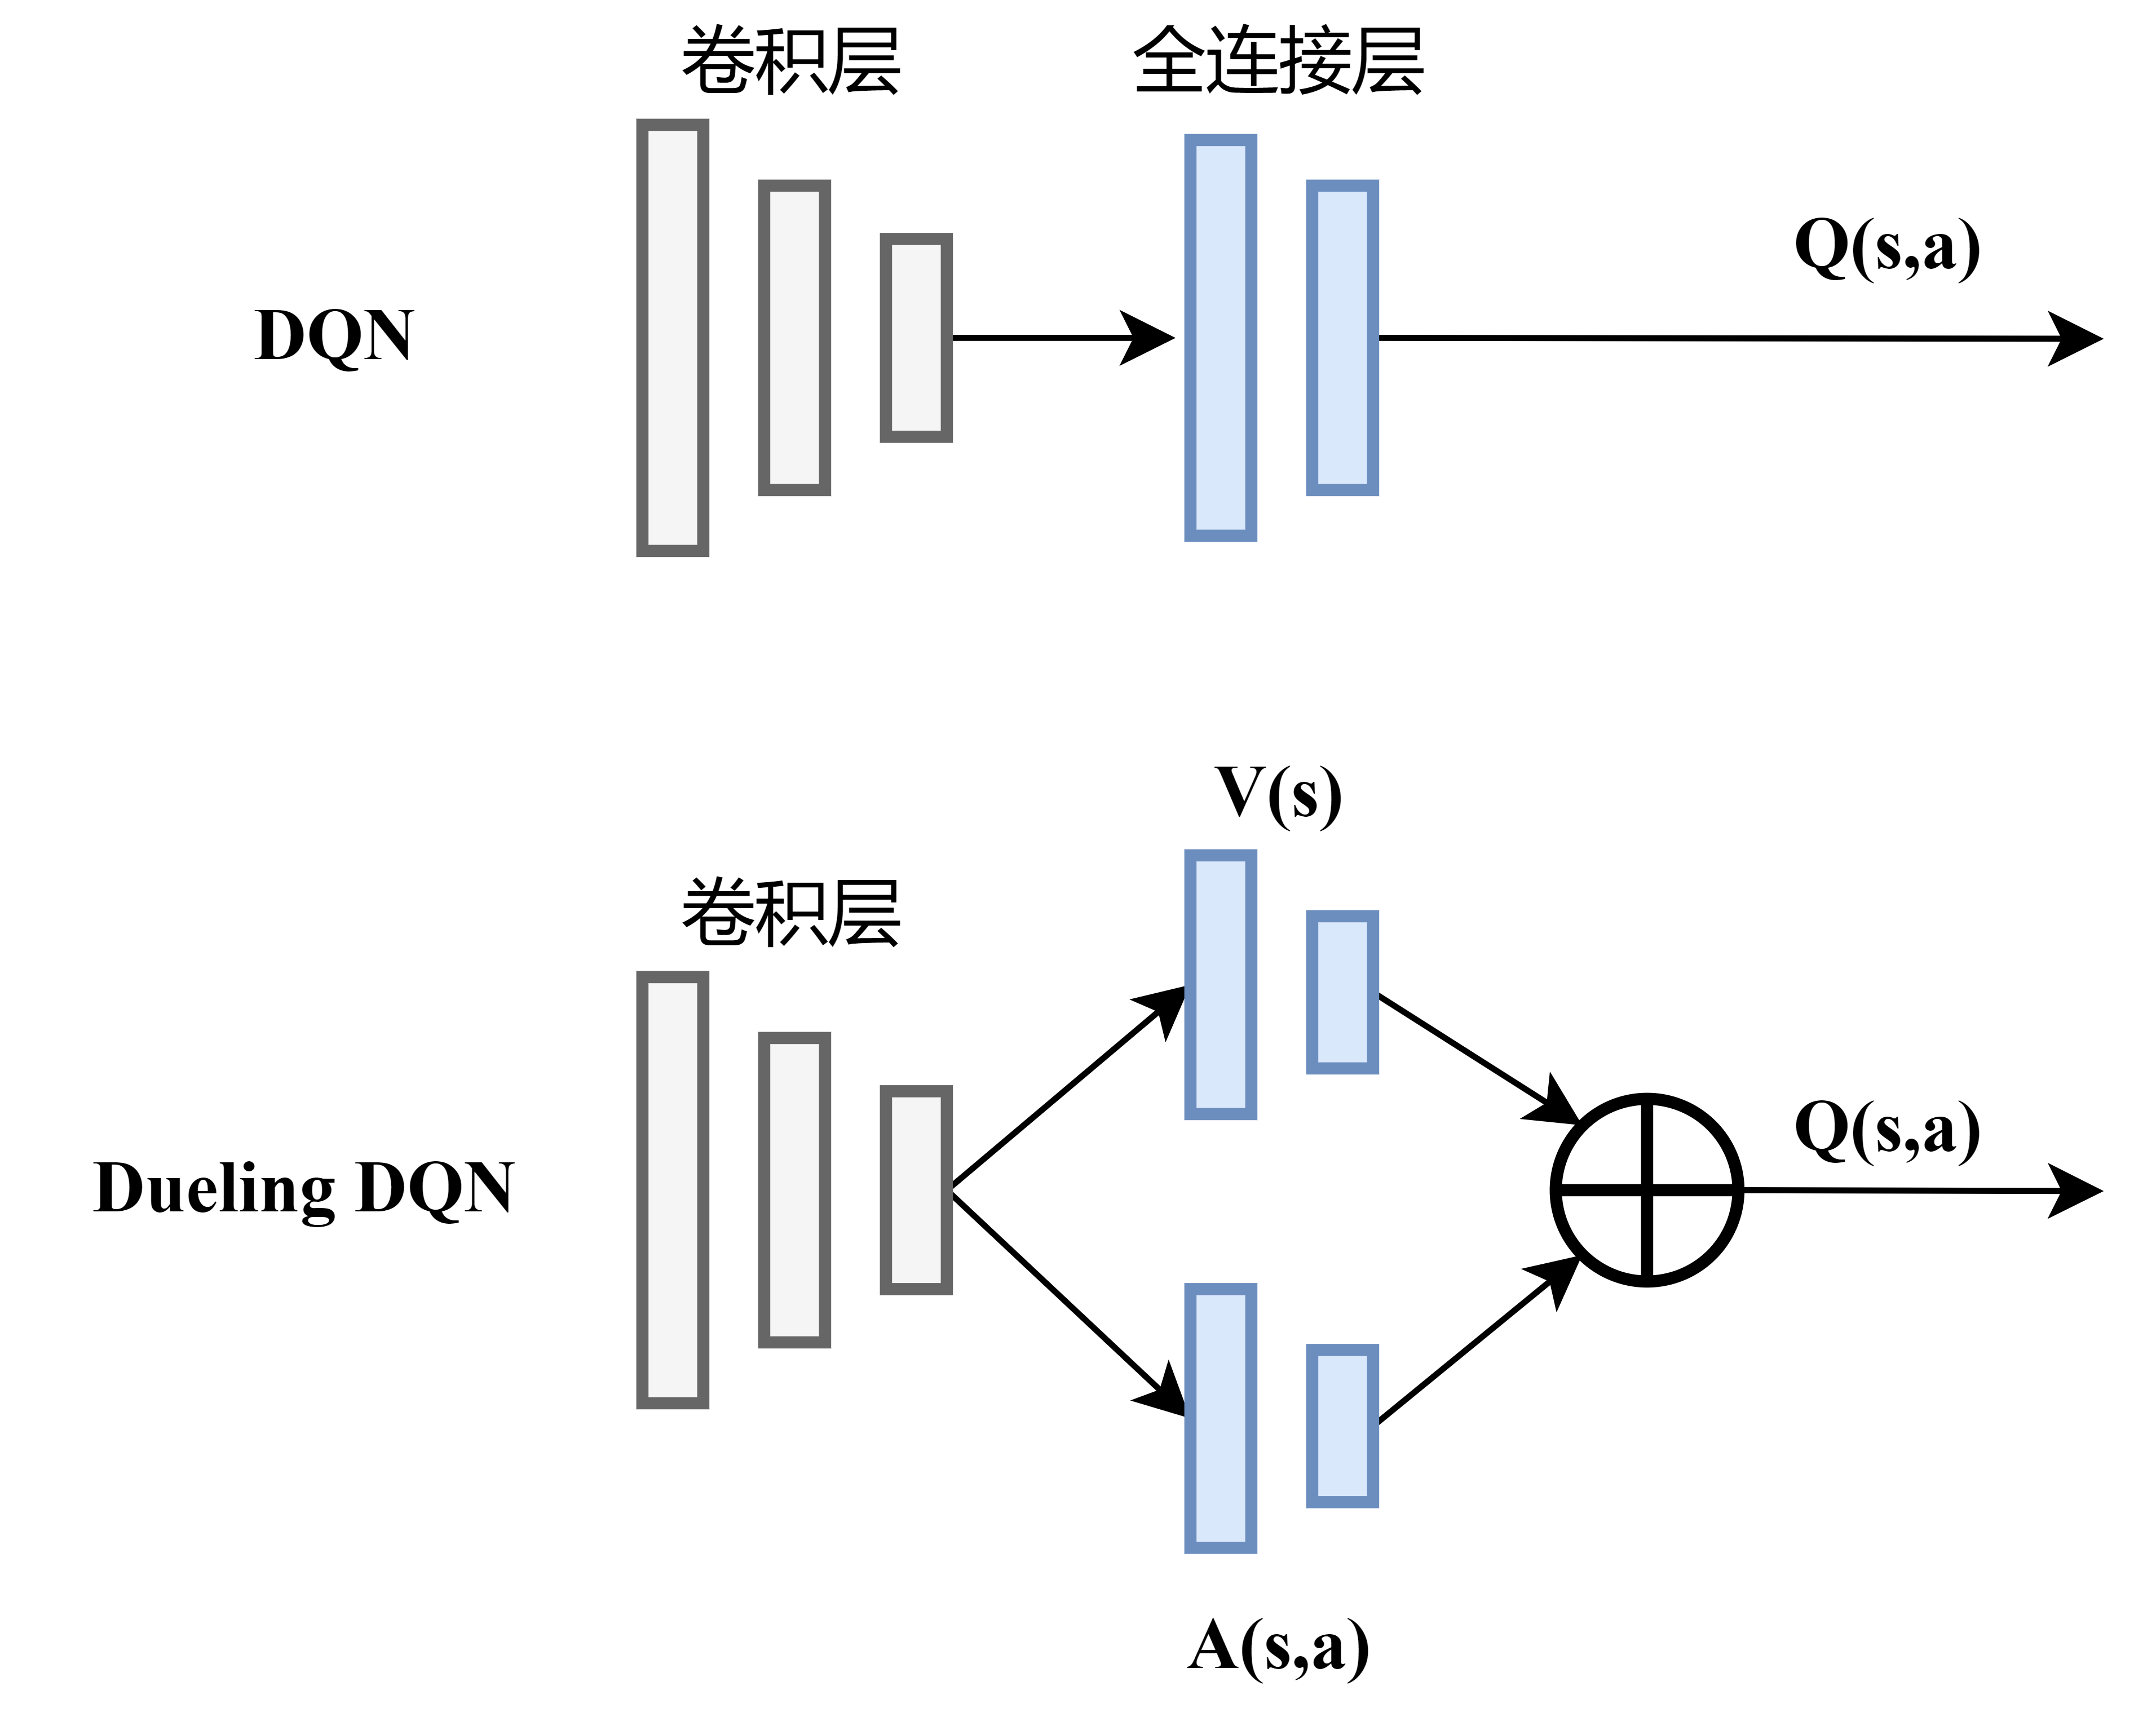
\includegraphics[width=0.63\textwidth]{images/chapter2/Dueling_DQN.png}
    \caption{DuelingDQN网络结构}\label{DuelingDQN网络结构} % label 用来在文中索引
\end{figure}

Dueling DQN将卷积层提取的抽象特征分流到两个支路上,两个支路所采用的全连接层结构相同。两个支路分别输出状态值函数$V(s)$和优势值函数$A(s,a)$,聚合函数将两个支路合并为Q函数:
\begin{equation*}
    Q(s,a;\alpha,\beta) = V(s;\beta) + A(s,a;\alpha)
\end{equation*}
但此式存在一个无法识别的问题,在确定的Q下,V和A有无数可能,故需要对A值做出限定,强制令所有选择贪婪动作的优势函数为0(认为没有比选择贪婪动作的方法更优的选项了)。添加约束条件,此时Dueling DQN的行为值函数为:
\begin{equation}
    Q(s,a;\alpha,\beta) = V(s;\beta) + A(s,a;\alpha) - \max_{a^{'} \in A}A(s,a^{'};\alpha)
\end{equation}

在实际中,一般使用优势函数的平均值代替上述最优值,虽然平均值改变了优势函数的值,但它可以保证缩小Q值的范围,去除多余的自由度,从而提高算法的稳定性。
\begin{equation}
    Q(s,a;\alpha,\beta) = V(s;\beta) + A(s,a;\alpha) - \frac{1}{\left | A \right | } \sum_{a^{'} \in A}A(s,a^{'};\alpha)
\end{equation}

由于Dueling DQN与传统DQN有相同的输入输出,只需要改变网络结构和前向传播的公式,除此之外算法的处理流程和DQN是相同的。

\section{本章小结}% 讲一下要用DQN、DDQN和Dueling DQN来干一些事情。

本章介绍了强化学习算法的组成及其马尔科夫决策模型的求解,通过对基于值函数(Value Based)的Q-learning算法及DQN算法的详细分析,由于自动驾驶决策控制任务无法进行精确的“查表”预知,需要进行神经网络的拟合,故采取基于DQN及其改进算法Double DQN和Dueling DQN算法完成自动驾驶决策控制任务。同时,根据输入数据的抽象程度,下一章节将对三种DQN算法进行决策与控制方面的设计与探究,从而得到DQN及其改进算法的对比实验效果。
